\documentclass[10pt]{article}
\usepackage{graphicx}

\begin{document}

\begin{figure}[h]
\caption{Model output: With rate of reproduction doubled} \label{fig:supp31} 
    \centering
    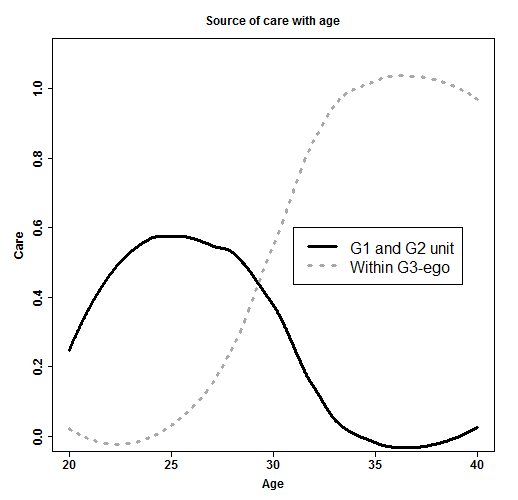
\includegraphics[scale=0.65]{repro_50per}

{Plot compares the mean amount of care distributed outside the focal unit to the amount of care given by older siblings across age.}
\end{figure}

\begin{figure}[h]
\caption{Model output: With an additional sister} \label{fig:supp32} 
    \centering
    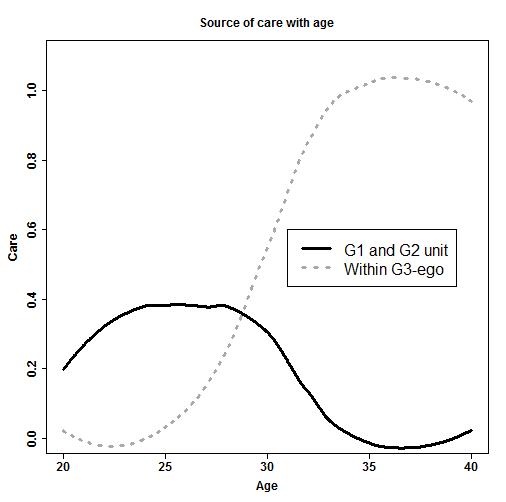
\includegraphics[scale=0.65]{third_sister}

{Plot compares the mean amount of care distributed outside the focal unit to the amount of care given by older siblings across age.}
\end{figure}

\begin{figure}[h]
\caption{Model output: Delaying transition from ``needy'' to ``caring'' until age 10} \label{fig:supp33} 
    \centering
    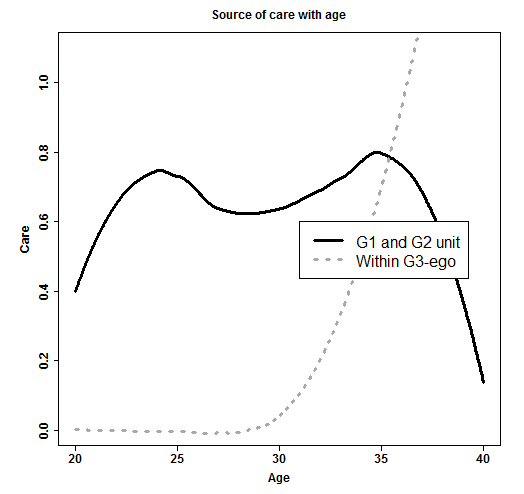
\includegraphics[scale=0.65]{need_till_10}

{Plot compares the mean amount of care distributed outside the focal unit to the amount of care given by older siblings across age.}
\end{figure}

\end{document}